\chap{Final Project}

\section{Objectives}
In this project, you are required to use the Altium Designer to design and layout a circuit that synthesize many knowledge that you have learnt in this course. There is something new, but no worries, we support you. 

The project will include 
\begin{itemize}
    \item how to design a digital input switches,
    \item how to use a diode to prevent a short-circuit,
    \item how to use a transistor generating a high current signal,
    \item how to use an opamp as a buffer and a low-pass filter before reading an ADC signal, and
    \item how to connect all the input and output signals to a micro-controller.
\end{itemize}

\section{Specifications}
In this project, you aim to design a circuit that is able  
\begin{itemize}
    \item to measure the current of an 220V AC signal,
    \item to set an address to distinguish with other similar circuits, up to 16, 
    \item to measure the maximum current either up to 5A or up to 10A,
    \item to send data to a gateway via RS485 or Wifi or Bluetooth,
    \item  (optional) to display on 7 segment LEDs using IC 74HC595.
\end{itemize}

\section{Solution}
To fulfill the requirements above, one of the solutions that we can think of is that 

\begin{itemize}
    \item We will use a current sensor [1] to measure the current of the AC signal. The sensor should support to measure up to 5A or up to 10A. There are many current sensors that are available in the market, we recommend you to use TA12 [2] for 5A maximum and TA17 for 10A maxumun. They are cheap and easy to use. 

    \item We will use 4 slide switches to set a board address. 
    
    \item We will use an IC that can convert from UART signals to RS485 signals [3] for transferring data via RS485.
    
    \item We will use a micro-controller (MCU) board, namely ESP32-WROOM-32 [4] as a main processor. ESP32-WROOM-32 is a powerful, generic WiFi and Bluetooth MCU module which is suitable to many IoT application. 

\end{itemize}

Now we list all the part that is required for our circuit. Based on the solution above, the circuit should include
\begin{itemize}
    \item A power supply input with the range of 5V - 36V,
    \item A regulator 3.3V to supply power to the module ESP32-WROOM-32,
    \item A microcontroller board ESP32-WROOM-32,
    \item A TA12/TA17 sensor that supports up to 5A or up to 10A,
    \item Slide switches for a board address,
    \item LEDs for display status,
    \item a RS485 circuit,
    \item and some capacitors for filtering noise.
\end{itemize}

\section{Guidance}
In this section, we give you some guidance to draw a circuit with the solution above. 

\subsection{Design a 3.3V regulator}
\begin{figure}[!htp]
    \centering
    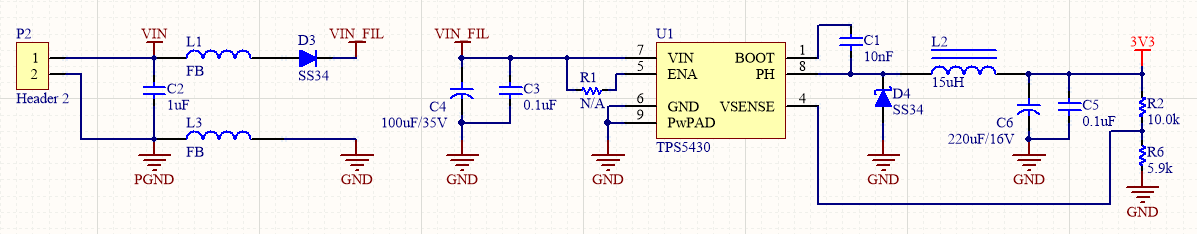
\includegraphics[width=6in]{source/picture/bai_7/bai7_power_supply.png}
    \caption{\textit{Power supply 3.3V regulator}}
    \label{bai7_power_supply}
\end{figure}

Figure \ref{bai7_power_supply} shows a power supply part for this circuit. It generates a 3.3V output for our circuit from input from 5V-36V to 3.3V. On the left, P2 is a input header which 5-36V input is coming. The input power supply goes through a LC circuits (L1, L3 and C2) to filtering the high frequency noises. Then it goes though a diode D3 which is used to prevent the error from input at P2. Finally, we use IC TPS5430 [5] to generate a voltage 3.3V output. 
\newpage
\subsection{Design a ESP32-WROM-32 part}
\begin{figure}[!htp]
    \centering
    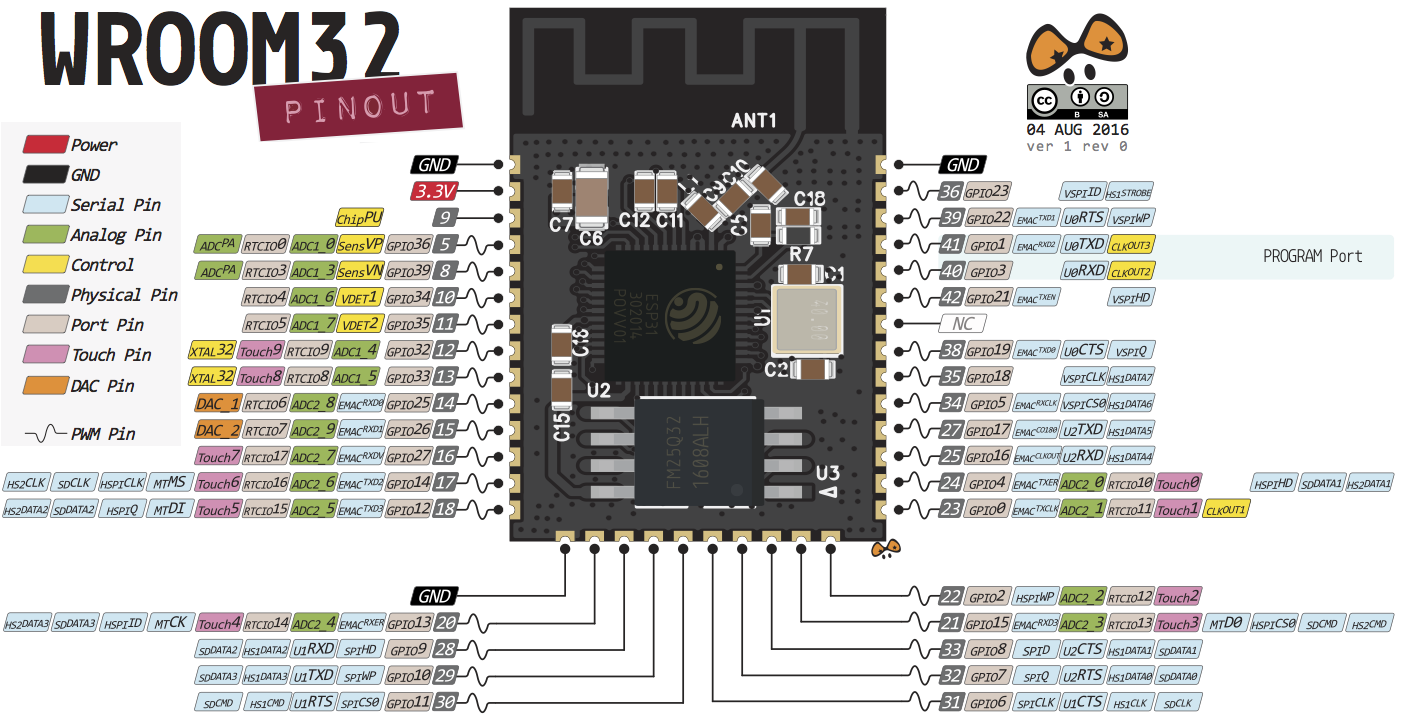
\includegraphics[width=5in]{source/picture/bai_7/bai7_esp32_pinout.png}
    \caption{\textit{ESP32-WROOM-32 pinout}}
    \label{bai7_esp32_pinout}
\end{figure}

Figure \ref{bai7_esp32_pinout} shows the pinout of the board ESP32-WROOM-32. 
It has on board 18 Analog to digital conversions (ADCs).  Each ADC is 12 bit SAR technology based.
2 digital to analog conversion (DACs). It integrates 9 touch sensors.
For communication, it has 2 UART communications channels, 2 I2C communications interfaces, two I2S channels and one CAN communication interface.
It has 16 pulse width modulation channels.
It also has a cryptographic hardware acceleration module for various cryptographic algorithms like RSA, AES.


\begin{figure}[!htp]
    \centering
    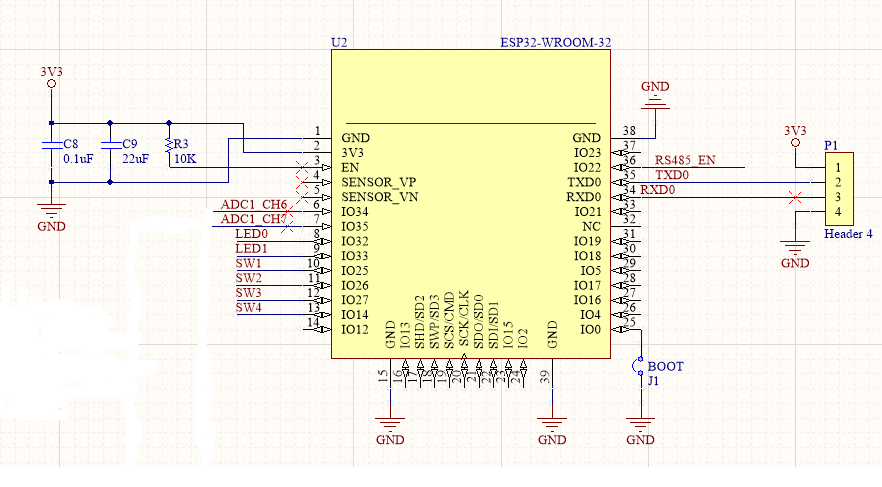
\includegraphics[width=5in]{source/picture/bai_7/bai7_mcu.png}
    \caption{\textit{ESP32-WROOM-32}}
    \label{bai7_mcu}
\end{figure}
To fulfill the solution above, we will use 2 pins for ADC inputs, 2 pins for LEDs, 4 pins for switches and 3 pins for RS485 as shown in Figure \ref{bai7_mcu}.
\newpage

\subsection{Interfacing Slide Switch with an MCU}
\begin{figure}[!htp]
    \centering
    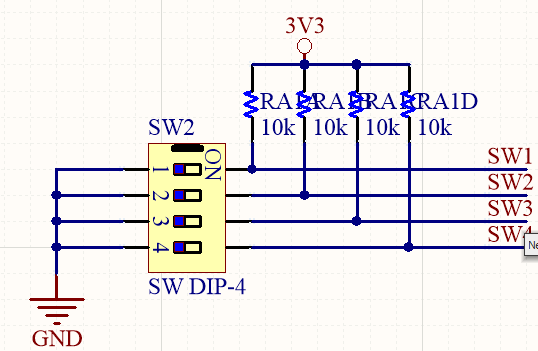
\includegraphics[width=3in]{source/picture/bai_7/bai7_switches.png}
    \caption{\textit{Switches}}
    \label{bai7_switches}
\end{figure}
We use a SW DIP-4 for 4 switches which each switch has two terminals. One terminal connects with ground and the other connects with a resistor to 3.3V power supply and connects to the MCU pins. For resistors you can use 4 single resistors or you can use a RAID including 4 resistors inside.

\newpage
\subsection{Current sensor circuit}
In this sensor part, we use two opamps which are packed in one IC LM358. IC LM358 includes two opamps. We use one to create a reference voltage, while we connect the second opamp with two current sensor TA12 and TA17 as shown in Figure \ref{bai7_ADC_Input}.
\begin{figure}[!htp]
    \centering
    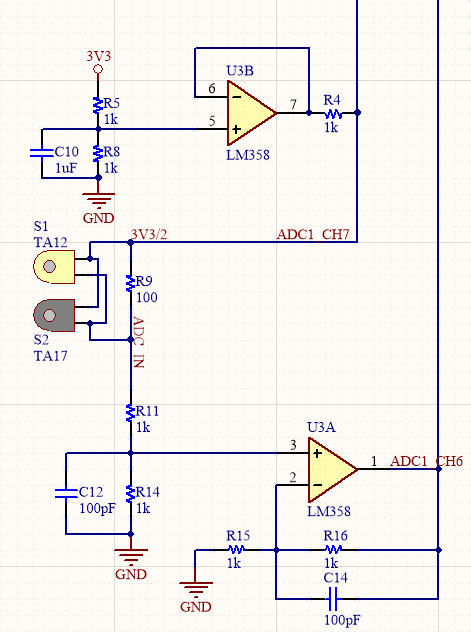
\includegraphics[width=4in]{source/picture/bai_7/bai7_ADC_Input.png}
    \caption{\textit{ADC Input}}
    \label{bai7_ADC_Input}
\end{figure}

\newpage
\subsection{Design a RS-485 part}
\begin{figure}[!htp]
    \centering
    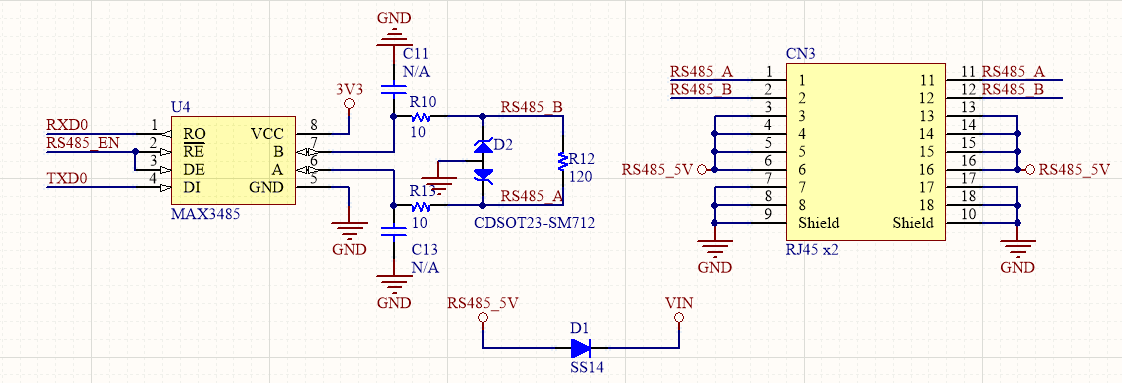
\includegraphics[width=6in]{source/picture/bai_7/bai7_rs485.png}
    \caption{\textit{RS 485}}
    \label{bai7_rs485}
\end{figure}
For RS-485 part, we use an IC MAX485 to convert UART signal to 485 signal and vice versa. We also use a RJ45x2 to connect RS-485 signals. Last thing we need to consider for this part is that RJ45x2 is also supply 5V input, so we use D1 to prevent the current go through the RS485\_5V pins. 

\newpage
\subsection{Interface with high-current LEDs}
Now, we design an output part which includes a 2-color LED as shown in Figure \ref{bai7_LEDs}. In this part, we use two transistors to connect with the 2-color LED.
\begin{figure}[!htp]
    \centering
    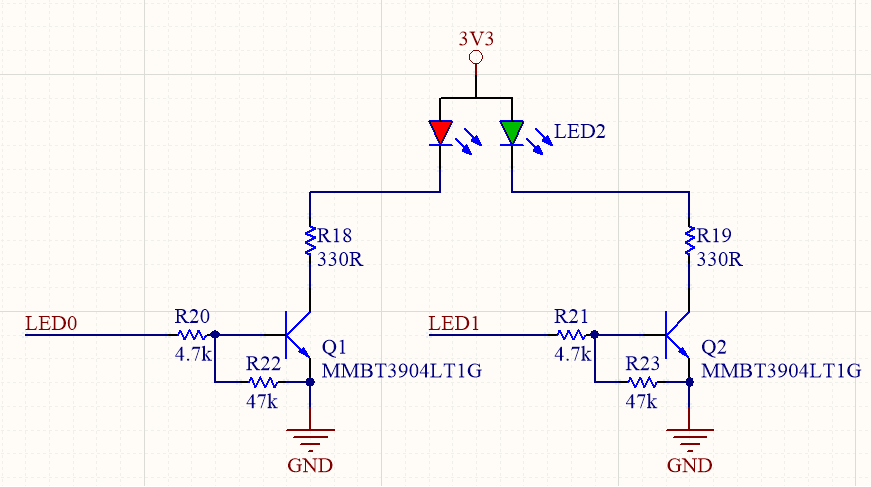
\includegraphics[width=5in]{source/picture/bai_7/bai7_LEDs.png}
    \caption{\textit{LED display}}
    \label{bai7_LEDs}
\end{figure}
%\subsection{Design a 2-button part}
%\subsection{(Optional)Design a 7-segment LED part}

\newpage
\section{Example of a final result}
Here is the sample of final result that you can use as a reference. 
\begin{figure}[!htp]
    \centering
    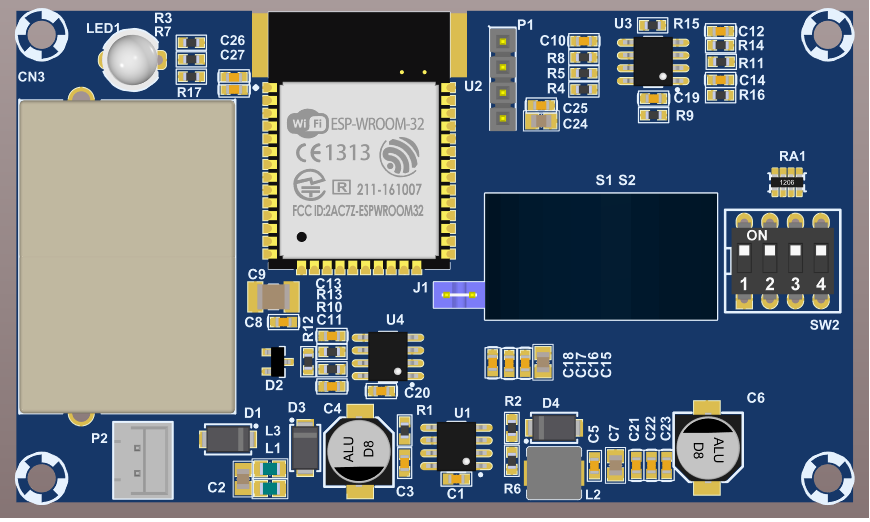
\includegraphics[width=5in]{source/picture/bai_7/bai7_3d_1.png}
    \caption{\textit{Final result 1}}
    \label{bai7_3d_1}
\end{figure}

\begin{figure}[!htp]
    \centering
    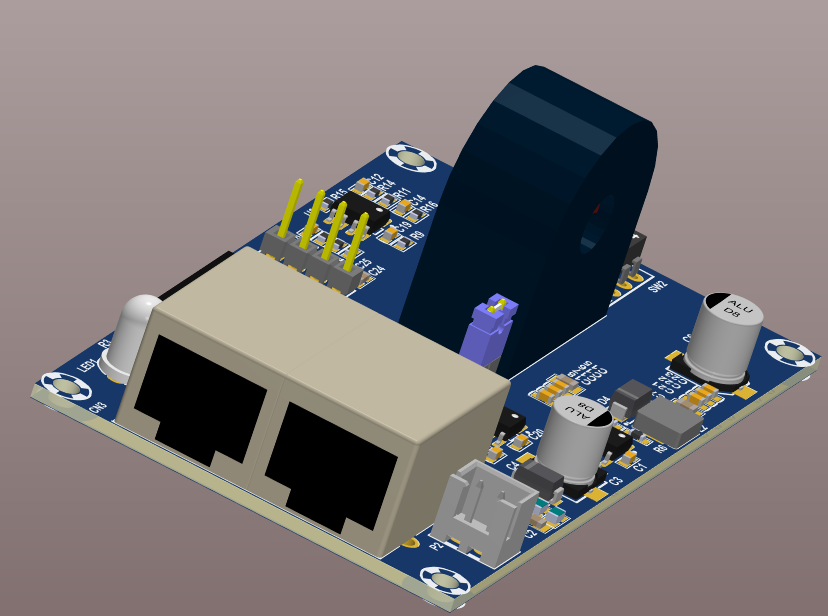
\includegraphics[width=5in]{source/picture/bai_7/bai7_3d_2.png}
    \caption{\textit{Final result 2}}
    \label{bai7_3d_2}
\end{figure}

\newpage
\section{Requirements}
\subsection{Questions to answer}
[1] Research on the Internet and list 5 different current sensors that you can find. Along with each current sensor, please (1) give a reference source, (2) maximum current that the sensor can measure, and (3) how to obtain its values (e.g, using ADC, UART, I2C or SPI and so on). 

[2] In Figure \ref{bai7_switches}, what is the voltage of SW1 when slide switch 1 is ON? and is OFF? 

[3] In Figure \ref{bai7_ADC_Input}, what is the voltage of ADC1\_CH7? of ADC1\_CH6? 
    
[4] In Figure \ref{bai7_ADC_Input}, we apply a low pass filter to the signal ADC\_IN. What is the cutoff frequency of this low pass filter? If we want to set a cutoff frequency is about 10kHz, what should we change in the circuit of U3A? 

[5] How much do the currents go through each LED in Figure \ref{bai7_LEDs}? What should we do if we want to control a 100mW LED? 

[6] What is the main purpose of D2 in Figure \ref{bai7_rs485}?

[7] (Optional) How to use IC 74HC595 to design a circuit to display value on 4 7-segment LEDs?

\subsection{Requirements of your design and layout}
1. Please download this rule 
\textbf{https://bit.ly/3bV7Vdy}, import it to your Altium Design project. Then you can place and route as normal. 

2. Please note that the name of each component is shown in the figures above. You can use those information to search corresponding components on your project. All the components can be found in the \textbf{chipfc\_altium\_libs}, and also this library \\
\textbf{https://drive.google.com/file/d/1JEiZ35lH3vG2xTBQqrG1bsEvJScXG6Eq/view?usp=sharing}

3. Please make the board as small as possible. 


\newpage
\section{References}
[1] https://en.wikipedia.org/wiki/Current\_sensing

[2] http://www.electronicoscaldas.com/datasheet/TA12-TA12L-Series\_YHDC.pdf

[3] https://en.wikipedia.org/wiki/RS-485

[4] https://www.espressif.com/sites/default/files/documentation/esp32-wroom-32\_datasheet\_en.pdf
[5] https://www.ti.com/product/TPS5430